\section{Apéndices}

\subsection{Apéndice A}

Consideremos la secci\'on horizontal de un horno de acero cil\'\i ndrico,
como en la Figura 1. El sector A es la pared del horno, y el sector B es el
horno propiamente dicho, en el cual se funde el acero a temperaturas
elevadas. El borde externo de la pared es un c\'\i rculo, pero el borde
interno de la pared -que coincide con el borde del sector B- no
necesariamente tiene forma circular. Inicialmente lo consideraremos tambi\'en circular.

Supondremos que la temperatura del acero dentro del
horno es constante e igual a 1500 \grad C. Hay sensores ubicados en la pared externa del horno para medir la temperatura, y estos habitualmente indican una temperatura entre 50 \grad C  y 200 \grad C.

El problema que debemos resolver consiste en estimar la isoterma de 400 \grad C dentro de la pared del horno, para estimar la resistencia de la pared al momento de su puesta en marcha. Si esta isoterma est\'a muy cerca de la pared externa del horno, existe peligro de que la estructura externa de la pared colapse.

\begin{figure}[h]
\centering
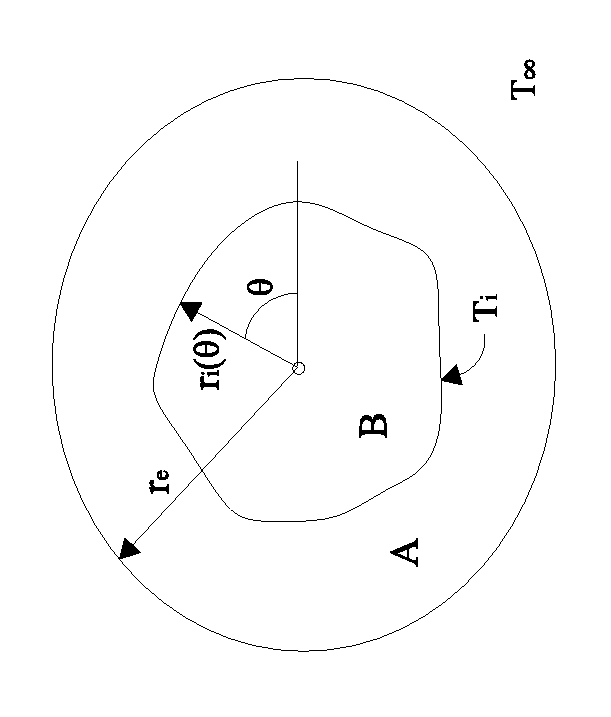
\includegraphics[scale=0.25,angle=-90]{../img/tp2.png} \\
Figura 1: Secci\'on del horno \\
\end{figure}


El objetivo del trabajo pr\'actico es implementar un programa que calcule la isoterma solicitada, conociendo las dimensiones del horno y las mediciones de temperatura en la pared exterior.

\textbf{El modelo}

Sea $r_e\in\real$ el radio exterior de la pared y sea $r_i:[0,2\pi]\to\real$
el radio interior de la pared, que suponemos dependiente del \'angulo (de
manera tal que $r_i(\theta)$ es la distancia desde el centro hasta el
borde del sector B en el \'angulo $\theta\in[0,2\pi]$). Llamemos $T(r,\theta)$
a la temperatura en el punto dado por las coordenadas polares $(r,\theta)$,
siendo $r$ el radio y $\theta$ el \'angulo polar de dicho punto. En el estado
estacionario (luego de un tiempo suficientemente largo de operaci\'on del
horno), esta temperatura satisface la ecuaci\'on del calor:
\begin{equation}
\frac{\partial^2 T(r,\theta)}{\partial r^2} + \frac{1}{r}
\frac{\partial T(r,\theta)}{\partial r} + \frac{1}{r^2}
\frac{\partial^2 T(r,\theta)}{\partial \theta^2} \ =\ 0 \label{calor}
\end{equation}
Llamemos $T_i\in\real$ a la temperatura en el interior del horno (sector B) y $T_e\in\real$
a la temperatura en el extrior de la pared. Las condiciones
de contorno del problema est\'an dadas por:
\begin{eqnarray}
T(r,\theta) & = & T_i \label{interior},  0<r\leq r_i \\[4pt]
T(r_e,\theta) & = & T_e(\theta) \label{exterior} 
\end{eqnarray}

La condici\'on (\ref{interior}) especifica que la temperatura en el borde
interior del horno debe ser igual a la temperatura del acero en fundici\'on,
mientras que la condici\'on (\ref{exterior}) especifica que la temperatura debe ser igual a las indicaciones de las termocuplas sobre la superficie exterior del horno.

El problema en derivadas parciales dado por la ecuaci\'on (\ref{calor})
con condiciones de contorno (\ref{interior}) y (\ref{exterior}) permite
encontrar la funci\'on $T$ de temperatura en la pared del horno (sector A),
en funci\'on de los datos mencionados en esta secci\'on.

\textbf{La resoluci\'on}

Para resolver este problema computacionalmente, discretizamos el dominio
del problema (el sector A) en coordenadas polares. Consideremos una
partici\'on $0=\theta_0 < \theta_1 < \dots < \theta_n = 2\pi$ en $n$
\'angulos discretos con $\theta_k - \theta_{k-1} = \Delta\theta$ para
$k=1,\dots,n$, y una partici\'on $0 = r_0 < r_1 < \dots < r_m = r_e$
en $m+1$ radios discretos con $r_j-r_{j-1} = \Delta r$ para $j=1,\dots,m$.

El problema ahora consiste en determinar el valor de la funci\'on $T$ en los
puntos de la discretizaci\'on $(r_j, \theta_k)$ que se encuentren dentro
del sector A. Llamemos $t_{jk} = T(r_j, \theta_k)$ al valor
(desconocido) de la funci\'on $T$ en el punto $(r_j, \theta_k)$.

Para encontrar estos valores, transformamos las ecuaciones (\ref{calor})
y (\ref{exterior}) en un conjunto de ecuaciones lineales sobre las
inc\'ognitas $t_{jk}$, evaluando (\ref{calor}) en todos los puntos de la
discretizaci\'on que se encuentren dentro del sector A y evaluando
(\ref{exterior}) en todos los puntos de la discretizaci\'on que se encuentren
en el borde exterior de la pared. Al hacer esta evaluaci\'on, aproximamos
las derivadas parciales de $T$ en (\ref{calor}) y (\ref{exterior}) por medio
de las siguientes f\'ormulas de diferencias finitas:
\begin{eqnarray}
\frac{\partial^2 T(r,\theta)}{\partial r^2}(r_j,\theta_k) & \cong & \frac{t_{j-1,k} - 2t_{jk} + t_{j+1,k}}{(\Delta r)^2} \nonumber \\[4pt]
\frac{\partial T(r,\theta)}{\partial r}(r_j,\theta_k) & \cong & \frac{t_{jk} - t_{j-1,k}}{\Delta r} \nonumber \\[4pt]
\frac{\partial^2 T(r,\theta)}{\partial \theta^2}(r_j,\theta_k) & \cong & \frac{t_{j,k-1} - 2t_{jk} + t_{j,k+1}}{(\Delta\theta)^2} \nonumber
\end{eqnarray}
Para cada \'angulo $\theta_k$, llamamos $g_k$ al menor radio tal que el
punto $(g_k, \theta_k)$ se encuentra dentro del sector A. Es importante
notar que el valor de la inc\'ognita $t_{g_k k}$ es conocido, dado que
en la discretizaci\'on el punto $(g_k, \theta_k)$ se encuentra sobre el
borde interior de la pared (es decir, $t_{g_k k} = T_i$).

Al realizar este procedimiento, obtenemos un sistema de ecuaciones lineales
que modela el problema discretizado. La resoluci\'on de este sistema permite
obtener una aproximaci\'on de los valores de la funci\'on $T$ en los puntos
de la discretizaci\'on.

\textbf{Enunciado}

Se debe implementar un programa que tome como entrada los datos del problema
y que calcule la temperatura en la pared del horno utilizando la t\'ecnica
de resoluci\'on descripta en la secci\'on anterior.

El programa debe tomar los datos de entrada desde un archivo de texto, cuyo
formato queda a criterio del grupo. Es importante mencionar que los
par\'ametros $n$ y $m$ de la discretizaci\'on forman parte de los datos
de entrada.

El programa debe generar el sistema de ecuaciones lineales planteado en
la secci\'on anterior, procediendo a su resoluci\'on por medio de cualquier
m\'etodo directo para la resoluci\'on de sistemas de ecuaciones lineales
(es decir, un m\'etodo no iterativo). El programa debe escribir la soluci\'on
en un archivo, con un formato adecuado para su posterior graficaci\'on.

Sobre la base del resultado del sistema de ecuaciones, el programa debe obtener la isoterma de 400 \grad C. El informe debe contener una descripci\'on detallada del m\'etodo computacional propuesto para obtener esta isoterma, junto con todas las decisiones que el grupo haya tomado con relaci\'on a este punto.

Se pide realizar experimentos con al menos dos instancias de prueba, generando distintas discretizaciones para cada una. Se recomienda fijar $r_e=1$ en estas instancias. Se sugiere que se presenten los resultados de estos experimentos en forma de gr\'aficos de temperatura o gr\'aficos de curvas de nivel, para ayudar a la visualizaci\'on de los resultados. Como objetivo adicional obligatorio, se pide graficar el tiempo de resoluci\'on en funci\'on del tama\~no de la discretizaci\'on, para predecir los tiempos en discretizaciones m\'as refinadas.
Finalmente, qu\'e espera que pase si el horno no presenta una geometr\'ia homogenea. Explicar en palabras c\'omo procedería a resolver el problema. 



\subsection{Apéndice B}
\label{sec:apendice}

\subsubsection{Código fuente que genera y resuelve el sistema de ecuaciones}

Incluimos a continuación el código (simplificado) relevante de las funciones usadas para generar y resolver el sistema de ecuaciones segun lo descripto en el desarrollo de este informe.

\begin{verbatim}

  cin >> cant_radios >> cant_angulos >> radio_int >> radio_ext;

  for(int i = 0; i<cant_angulos; i++){
  
    double temp;
    cin >> temp;
    temps_exterior.push_back(temp);
  }
    
  radio_dist = (radio_ext-radio_int) / (cant_radios-1);
  angulo_dist = 2*M_PI / cant_angulos;
  
  cant_ecus = cant_angulos * cant_radios;

  matrix.resize(cant_ecus);
  vecsol.resize(cant_ecus);
  
  for (int i = 0; i < cant_ecus; i++){
    vecsol[i] = 0;
  }


  inicializar_matrix();

  cout << "BEFORE GAUSS" << endl;
  imprimir_matrix(matrix);

  gauss(matrix);
  cout << "AFTER GAUSS" << endl;

  imprimir_matrix(matrix);

  vd res= resolver_triangulado(matrix, vecsol);

  for (unsigned int i =0; i< res.size(); i++ ){
    cout << "El valor x" << i << " es: " << res[i] << endl;
  }
    
  calcular_iso(res);

\end{verbatim}

\subsubsection{Código fuente de la eliminacion gaussiana}

Incluimos a continuación el código relevante que realiza la eliminacion gaussiana

\begin{verbatim}
  int tam = matrix.size();
  for (int i = 0; i < tam-1; i++){
    for (int k = i+1; k < tam; k++){
      if (matrix[k][i] != 0){
        double factor = matrix[k][i]/matrix[i][i];
        for (int j= 0; j < tam; j++){
          matrix[k][j] -= matrix[i][j]*factor;
        }
        vecsol[k] -= vecsol[i]*factor;
      }
    }
  }

\end{verbatim}

\subsubsection{Código fuente que resuelve la ecuación}

A continuacion se presenta el código relevante que resuelve la ecuación

\begin{verbatim}

  int tam = v.size();
  vd res(tam,0);
  res[tam-1] = v[tam-1];
  for (int i = tam-2; i >= 0; i--){
    if ((i>=cant_angulos) && (i<cant_ecus-cant_angulos) && (v[i] != r[i][i])){
      double acum = 0;
      for (int j = tam-1; j > i; j--){
        acum += r[i][j]*res[j];
      }
      acum-=vecsol[i];
      res[i] = acum / (-r[i][i]);
    }else{
      res[i] = v[i];
    }
  }
  return res;

\end{verbatim}

\subsubsection{Código fuente que calcula la isoterma}

Mas adelante incluimos el código relevante que calcula la isoterma

\begin{verbatim}

  vd res;
  vvd mat;
  mat.resize(cant_radios);
  
  for(int i =0; i<cant_radios; i++){
    mat[i].resize(cant_angulos);
  }
  
  for(int i =0; i<cant_radios; i++){
    for(int j =0; j<cant_angulos; j++){
      mat[i][j] = params[i*cant_angulos+j];
    }
  }
	
  for(int j =0; j<cant_angulos; j++){
    int i=0;
    while (mat[i][j]<400) i++;
    if (mat[i][j]==400){
      res.push_back(obtener_valor_radio(i));
    }else{
      double vmenor = mat[i-1][j];
      double vmayor = mat[i][j];
      double rmenor = obtener_valor_radio(i-1);
      double rmayor = obtener_valor_radio(i);
			
      double radio400 = rmenor + (400-vmenor)*(rmayor-rmenor)/(vmayor-vmenor);
			
      res.push_back(radio400);

    }
  }
	
  for (unsigned int i =0; i< res.size(); i++ ){
    cout << "La isoterma " << i << " es: " << res[i] << endl;
  }

\end{verbatim}